\chapter{System Design} \label{chapter:design}
% 在完成需求分析,导出完整的需求文档后,就可以对本项目进行系统设计工作了,系统设计是一项需要对系统功能,系统的输入与输出,系统的程序,系统的环境进行规约的工作,在进行系统设计时,需要考虑系统的经济性,可靠性,因此系统设计是一项重要的工作,决定了最终系统的质量\cite{systemdesignconcept}。在本章节,将使用UML用例图,类图以及系统结构图对项目进行系统建模。
After completing the requirements analysis and exporting the complete requirements document, the system design work can be carried out for this project. System design is a task that requires the specification of system functions, system inputs and outputs, system procedures, and system environment, and when carrying out system design, it is necessary to consider the economy and reliability of the system, so system design is an important task that determines the quality of the final system \cite{systemdesignconcept}. In this section, system modeling of the project will be performed using UML use case diagrams, class diagrams, and system structure diagrams.
\section{Use Case Diagram}
% 用例图可以粗略的定义系统与用户的交互行为,能够提供系统行为的概览\cite{rosenberg1999use}。本项目用例图包含了清洁电力电力用户,工厂用户,发电终端与系统的交互行为,主要是各类用户向系统提交交易请求,触发智能合约以向区块链中写入数据,改变系统状态的一系列行为,详尽的描述可以在看到\fref{fig:usecase}
The use case diagram can roughly define the interaction behavior between the system and users, and can provide an overview of the system behavior \cite{rosenberg1999use}. The use case diagram of this project contains the interaction behavior of clean power users, plant users, and power generation terminals with the system, mainly a series of behaviors in which various users submit transaction requests to the system, trigger smart contracts to write data to the blockchain, and change the system state, which can be described in detail in see \fref{fig:usecase}

\begin{figure}[!htb]
    \centering
    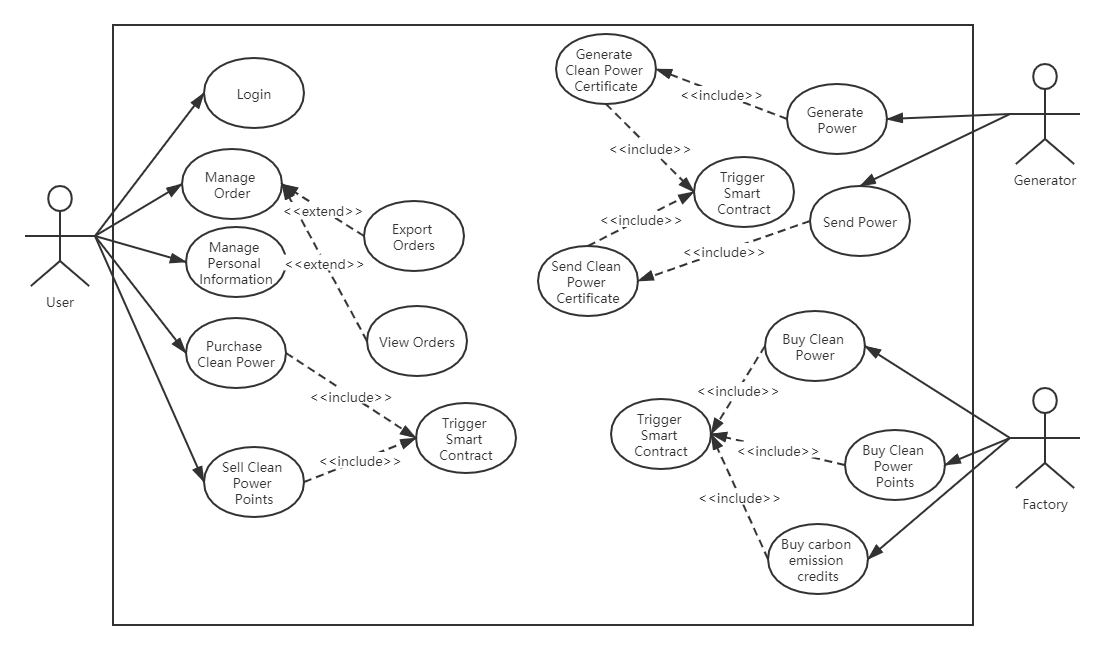
\includegraphics[width=\textwidth]{img/Usecaseforsummerproject.png}
    \caption{Use case diagram of the system}
    \label{fig:usecase}
\end{figure}

\section{Class Diagram}
% 通过类图,系统的实体之间的关系可以被清晰的观察到,本项目定义了用户,发电终端,清洁电力证书,订单,礼物,清洁电力积分,清洁电力等实体,类之间的关系和类的具体结构被\fref{fig:classdiagram}详细的表示了出来。
The relationship between the entities of the system can be clearly observed through the class diagram. This project defines entities such as user, generation terminal, clean power certificate, order, gift, clean power credit, clean power, and so on. The relationship between the classes and the specific structure of the classes are represented in detail by \fref{fig:classdiagram}.
\begin{figure}[!htb]
    \centering
    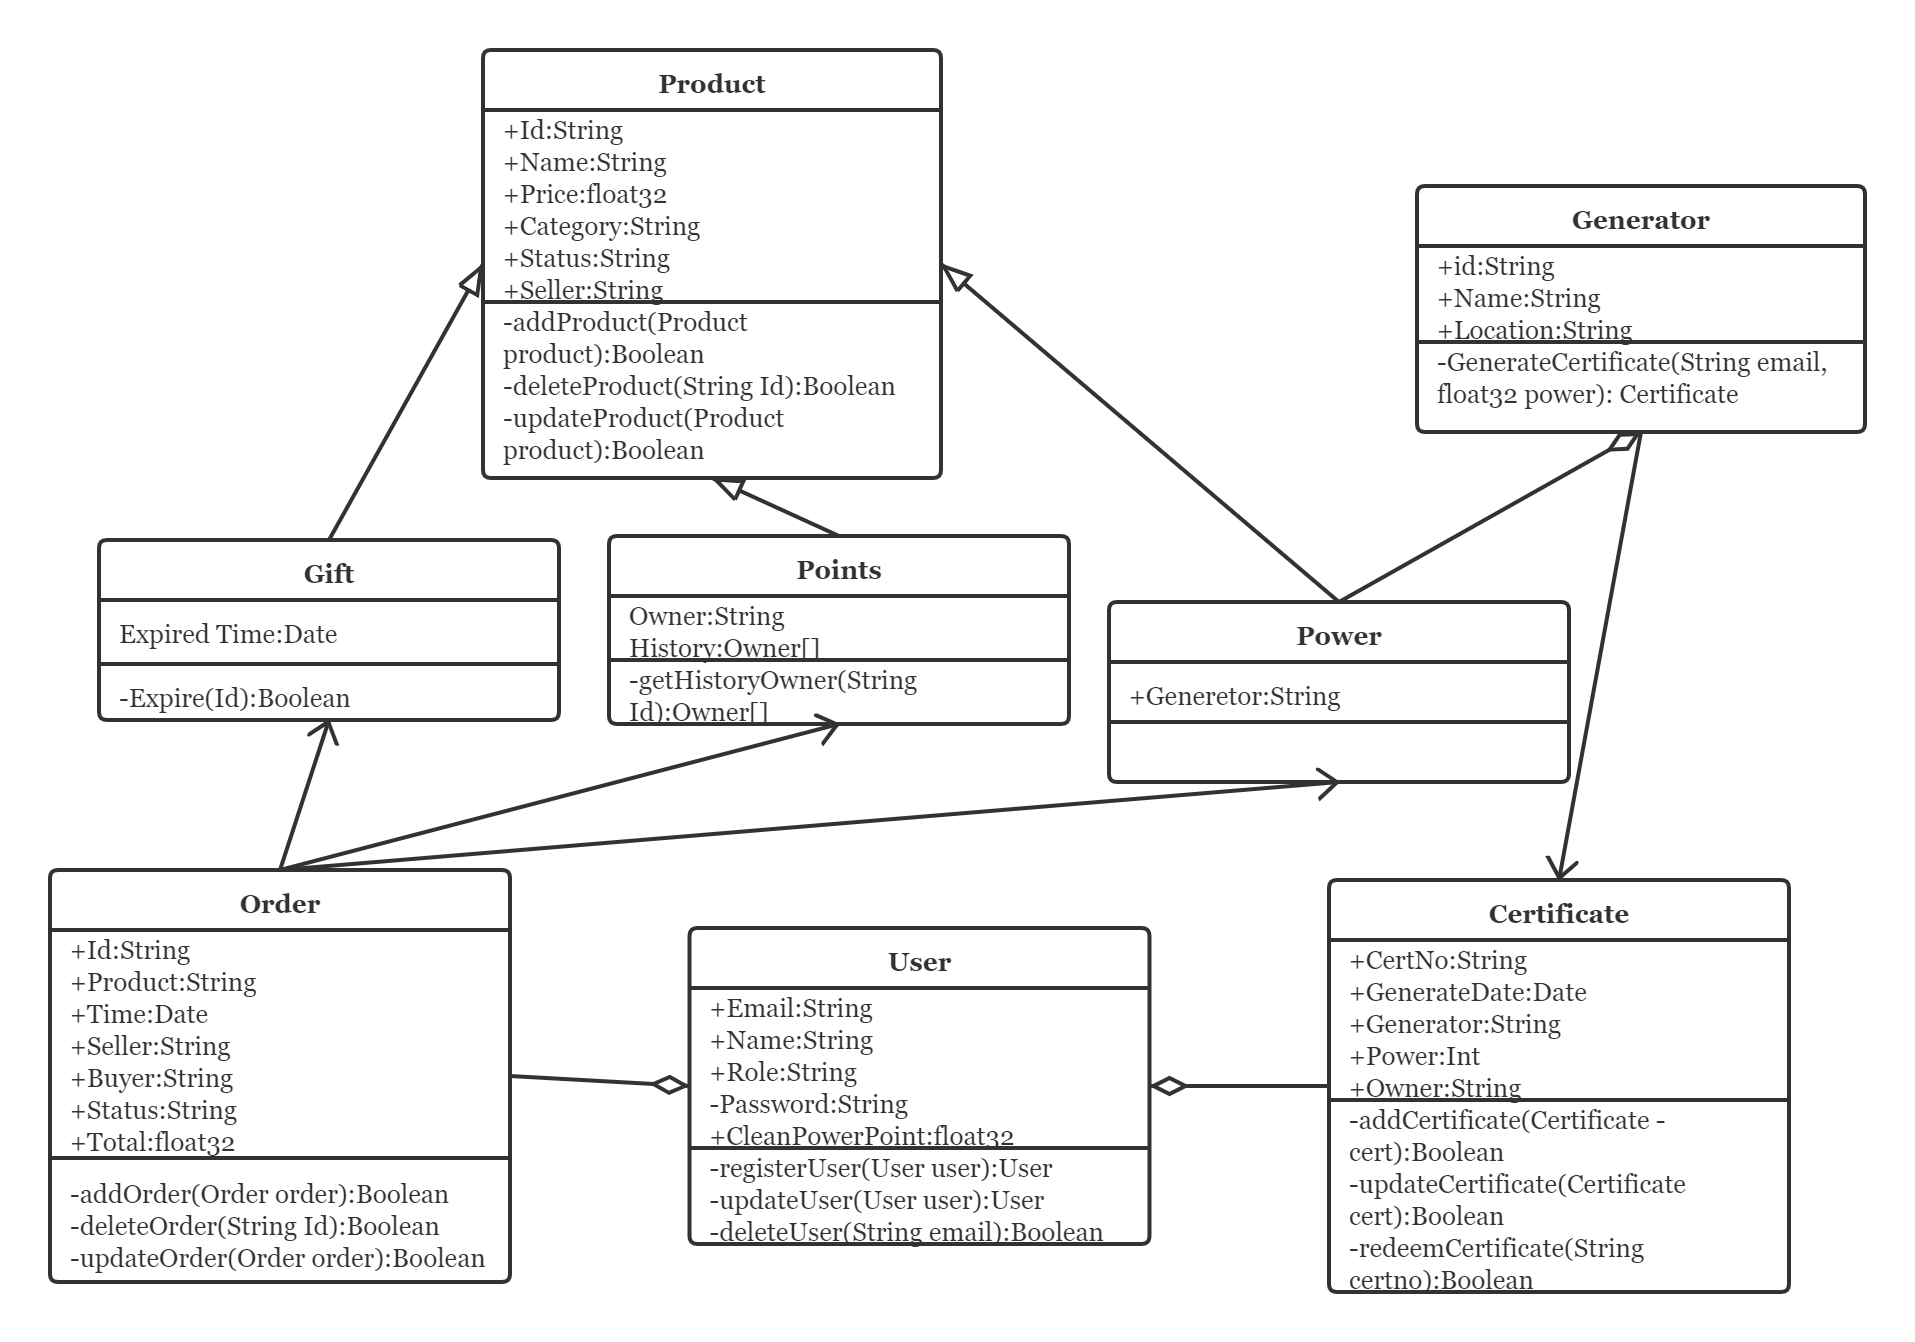
\includegraphics[width=\textwidth]{img/classdiagram.png}
    \caption{Class diagram of the system}
    \label{fig:classdiagram}
\end{figure}

\section{System Architecture}
% 为了能够快速高效的进行系统开发,在确定了系统用例以及实体之间关系之后,需要进行系统的架构设计,以便选择合适的实施方法,实施平台,从而进入实际的开发阶段,本项目选用Browser/Client结构,通过浏览器对区块链进行访问,使用Nodejs,Express,MongoDB,React实现传统的数据操作逻辑,使用Golang进行智能合约开发,将传统数据操作逻辑与智能合约通过Restful Api进行连接,最后对区块链进行操作。详细的系统结构如\fref{fig:sysarchtecture}所示。
In order to be able to develop the system quickly and efficiently, after determining the system use cases and the relationship between entities, the system architecture design is needed in order to select the appropriate implementation method and implementation platform, so as to enter the actual development phase, this project chooses Browser/Client structure, accessing the blockchain through the browser, choosing Nodejs, Express, MongoDB, React (MERN technology stack) to implement the traditional data operation logic, use Golang for smart contract development, connect the traditional data operation logic with the smart contract through Restful Api, and finally the smart contract will operate on the blockchain. The detailed system structure is shown in \fref{fig:sysarchtecture}.
\begin{figure}[!htb]
    \centering
    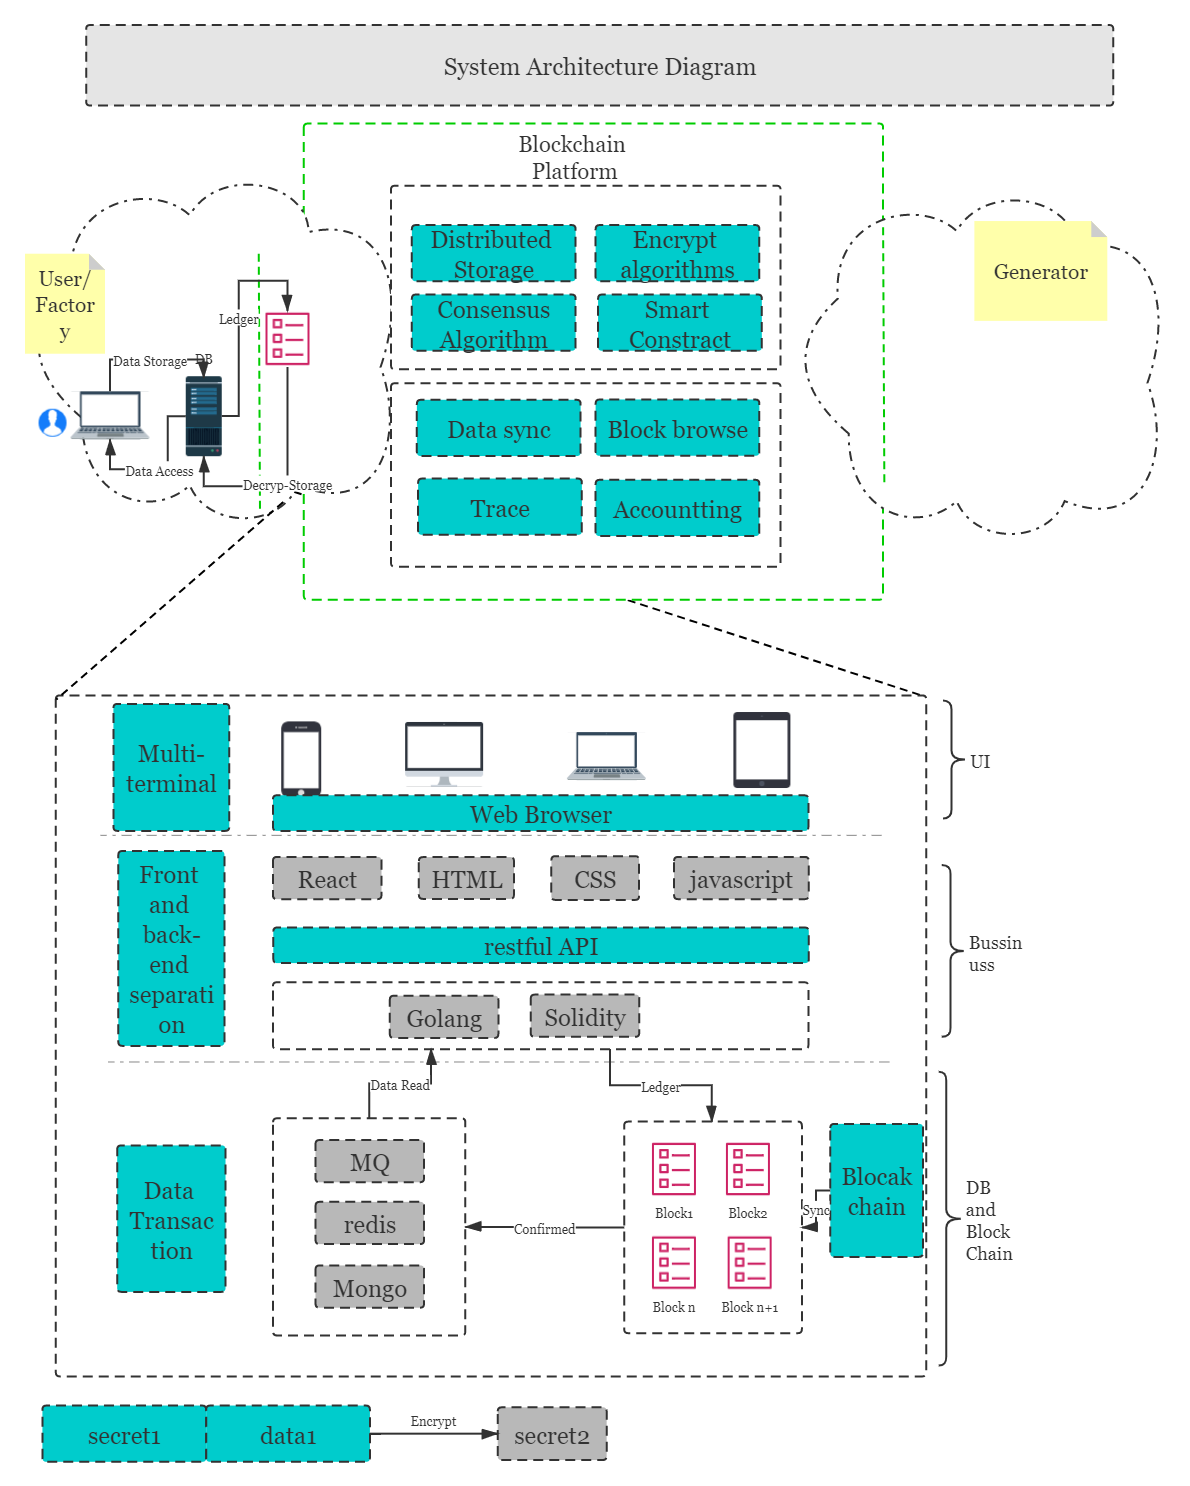
\includegraphics[width=.8\textwidth]{img/Architecture.png}
    \caption{System Architecture of the system}
    \label{fig:sysarchtecture}
\end{figure}


